\chapter{Einleitung}
\label{Kapitel:Einleitung}


\section{Überblick}
 
 Die Menge an analysierbaren  Informationen und den dazugehörigen Daten in Unternehmen nehmen immer stärker zu.  Durch den Zuwachs an Daten wird es aber auch immer schwieriger diese effektiv auszuwerten. Die  Daten in einzelnen und unterschiedlichen Programmen zu verwalten und zwischen diesen auszutauschen lässt sich zeitlich nicht mehr bewerkstelligen. Außerdem sind einige Datenquellen so stark angewachsen, das sie sich mit herkömmlichen Tabellenkalkulationsprogrammen nicht mehr auswerten lassen.
 
 
Es wird ein Umfeld bzw. System benötigt, welches diesen Ansprüchen gerecht wird. Ein Business Intelligence Umfeld mit einem zentralen Data Warehouse kann vielen dieser Anforderungen mehr als gerecht werden. Die neu aufgestellte Datenbasis steht dem gesamten Unternehmen zur Verfügung und führt so zu einer Vereinheitlichung der Datenstrukturen sowie deren Semantik. Eine funktionierende Business Intelligence erlaubt dem Unternehmen in kürzester Zeit, hochaktuelle Informationen und dynamische Berichte zu generieren, um flexibel am Markt agieren zu können. Komplexe Data Mining Anwendungen finden Muster in den Daten, um Geschäftsprozesse zu optimieren, die verborgenen Wünsche des Kunden aufzudecken oder völlig neue Geschäftsmodelle zu entwickeln.
 
Ziel dieser Arbeit ist es, einen fundierten Überblick über die Bedeutung der Business Intelligence, des Data Warehouse sowie dem Reporting in diesem Umfeld zu geben und am Ende mögliche Umsetzungsmöglichkeiten zu demonstrieren.
 
\section{ Aufbau der Arbeit}
 
Im zweiten Kapitel wird der Frage nachgegangen, was man überhaupt unter dem Begriff „Business Intelligence“ versteht und ob es eine Möglichkeit gibt, diesen genau zu definieren. Hierfür wird ein kurzer Überblick über die geschichtliche Entwicklung der Informationssysteme innerhalb der Unternehmen eingeschoben, der schließlich in einem Referenzmodell mündet. Dieses Modell zeigt, wie aktuelle BI-Landschaften aussehen könnten. Hier wird versucht zu erklären, wie ein Business Intelligence System funktioniert und welche Möglichkeiten man hat, dieses effektiv zu nutzen.
 
Das Konzept und die Funktionsweise eines Data Warehouse hat, aufbauend auf dem zweiten Kapitel, das dritte Kapitel zum Inhalt. Es versucht das allgemein anerkannte Data Warehouse Konzept und die darauf aufbauende Referenzarchitektur darzustellen und die Prozesse innerhalb des Data Warehouse entsprechend zu erläutern. Hierfür wird aufgeführt, welche Anforderungen an die Systeme zu stellen sind um dem analytischen Gedanken zu folgen. Das Kapitel wird mit einer Einführung in die multidimensionalen Datenmodelle und deren Abbildung im relationalen Umfeld abgeschlossen.
 
Kapitel 4 stellt die Erfordernisse eines Reportings dar und versucht die Thematiken Business Intelligence und Data Warehouse in dieses Thema zu integrieren. Es soll aufzeigen, wie sich die gewonnenen Erkenntnisse der vorherigen Kapitel schließlich auch im Bereich des Unternehmensreportings widerspiegeln. Hierzu orientiert sich das Kapitel an der Management Reporting Excellence, der Idealform des Management Reportings.
 
Abschließend soll das fünfte Kapitel aufzeigen, wie man mit Open Source Produkten ein Business Intelligence Umfeld aufbauen und administrieren kann. Es stellte sich heraus, dass es hier zu einigen Problemen kommen kann, die ebenfalls im Kapitel erläutert werden.
 
Die Arbeit endet mit einer Schlussbetrachtung, die abschließend aufzeigen soll, ob die Problemstellungen der einzelnen Kapitel gelöst worden sind und welche Fragen eventuell nicht beantwortet werden konnten.



\chapter{Begriffserläuterung}
\begin{description}
	\item [Data Warehouse bzw. Business Warehouse] ist eine von den operativen Datenverarbeitungssystemen separierte Datenbank, auf die nur Lesezugriff besteht. In regelmäßigen Abständen werden aus den operativen DV-Systemen unternehmensspezifische, historische und daher unveränderliche Daten zusammengetragen, vereinheitlicht, nach Nutzungszusammenhängen geordnet, verdichtet und dauerhaft in der Datenbasis des Data Warehouses archiviert. Ziel ist die Verbesserung der unternehmensinternen Informationsversorgung (Wissensmanagement) und damit der Unterstützung strategischer Entscheidungen. Als analytisches System liefert es Informationen zur Problemanalyse - Online Analytical Processing (OLAP) -, die durch die Anwendung von Methoden (z.B. des Data Mining) generiert werden.  \href{http://wirtschaftslexikon.gabler.de/Definition/data-warehouse.html?referenceKeywordName=Business+Warehouse}{\textbf{QUELLE}}
\end{description}




Was ist Buisness Warehouse und Data Warehouse kurze Definition \\
Ein Data Warehouse ist kein Produkt, sondern ein Konzept, das sich der Datenproblematik von managementunterstuetzenden Systemen annimmt\\
A data warehouse is a subject-oriented, integrated, nonvolatile, time-variant collection of data in support of management’s decision \\

1. subject-oriented: Die Themenausrichtung an Sachverhalten des Unternehmens, z.B. Kunden- oder Produktkriterien, wird im BW durch das konsequente Einordnen aller Daten in Fachbereiche und durch die Bezugnahme auf Geschäftsprozesse realisiert (Seemann/Schmalzridt/Lehmann 2001, 18). Im Gegensatz dazu sind operative Daten immer auf einzelne betriebliche Funktionen bezogen (Schinzer/Bange/Mertens 1999, 14 - Bange/ Schinzer o.J., 1). \\
2. integrated: Mit dem DW-Konzept wird eine unternehmensweite Integration von Daten in einem einheitlich gestalteten System angestrebt (Mucksch/Behme 2000, 11). Verein- heitlichung und Integration externer und interner Daten bedeutet weniger die physische Zentralisierung der Daten in einem einzigen Datenpool, sondern deren logische Ver- bindung. Integration bedeutet konsistente Datenhaltung im Sinne einer Struktur- und Formatvereinheitlichung durch Maßnahmen wie Vergabe eindeutiger Bezeichnungen, Anpassung der Datenformate und Herstellung einer semantischen Integrität (Mucksch/ Behme 2000, 11ff.). Ebenso tragen Elemente wie einheitliche Merkmale und standardi- sierte Kennzahlen zu einer Datenintegration bei.\\
3. nonvolatile: Bei einem DW handelt es sich um eine dauerhafte Sammlung von Informationen, auf die im Gegensatz zu OLTP-Systemen (online transaction processing3) nur in Form von Lese- und Einfügeoperationen zugegriffen werden darf, um die Nicht- Volatilität der Daten sicherzustellen.4 Dieser Forderung kann jedoch nur bedingt zuge- stimmt werden, da Korrekturen von aus Quellsystemen geladenen Daten auf jeden Fall möglich sein müssen (Behme 1996, 31). Das BW bietet hierfür eine Eingangsablage in Form der Persistent Staging Area (PSA)5, in der manuelle Korrekturen zur Validierung und Fehlerbehebung nach dem Extraktionsvorgang durchgeführt werden können (SAP 2000a, 1; SAP 2000b).\\
4. time-variant: Während bei operativen Systemen eine zeitpunktgenaue Betrachtung der Daten im Mittelpunkt steht, liegt das Interesse bei Auswertungen im DW eher in einer Zeitraumbetrachtung, z.B. einer Trendanalyse (Behme 1996, 31). Der Zeitraumbezug ist daher impliziter oder expliziter Bestandteil der Daten in einem DW. Ein Ansatz zur Herstellung dieses Zeitraumbezugs im BW ist die obligatorische Verwendung einer Zeitdimension in jedem Informationsspeicher.


\begin{figure}[H]
    \centering
    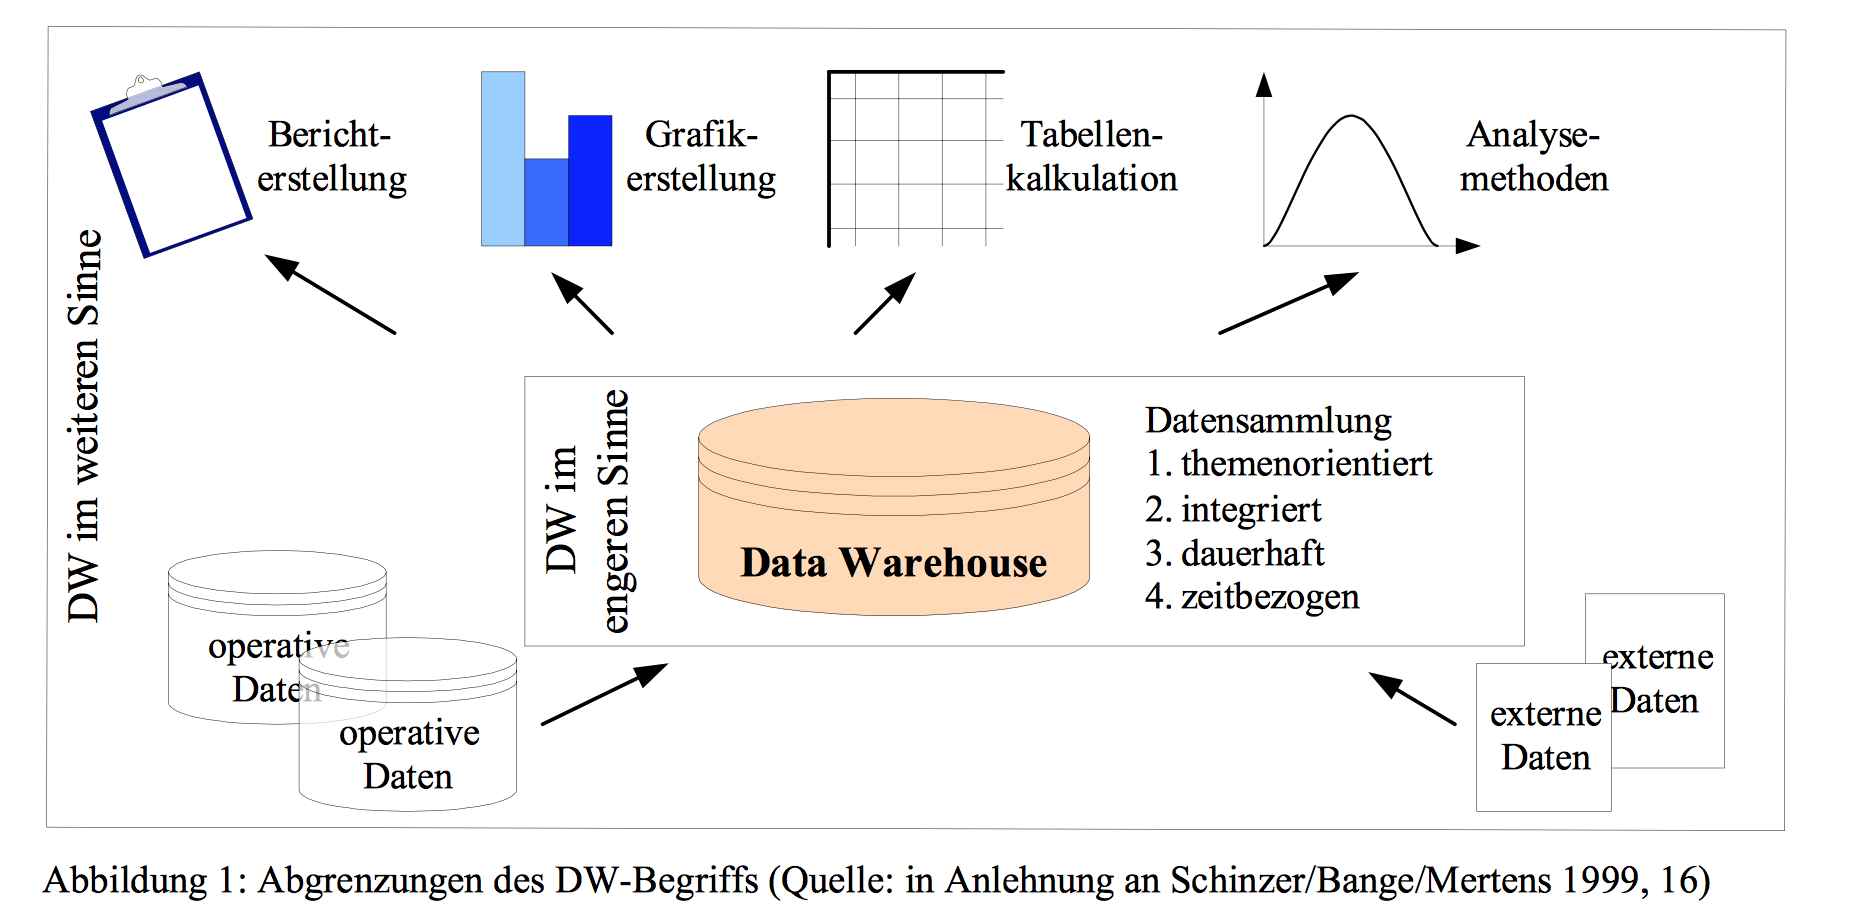
\includegraphics[width=1\textwidth]{files/DWOverview}
    \caption{Abgrenzungen des DW-Begriffs Q:(Schinzer/Bange/Mertens 1999, S.16)}
    \label{pic:DWOverview}
\end{figure}




Text
